\documentclass[../../Aurora C# unofficial manual.tex]{subfiles}

\begin{document}
	\section{Ground force logistics}
	Original post can be found
	\href{http://aurora2.pentarch.org/index.php?topic=8495.msg109760#msg109760}{here}.
	\\\\
	
	Ground Units have two separate logistics requirements. The first is Maintenance, which applies to all units at all times and has a wealth cost equal to 12.5\% of Ground Unit cost per annum. The second is Ground Supply Points (GSP), which applies only to combat units during ground combat.
	
	The GSP requirement for a weapon component is equal to \( Penetration Value * Damage Value * Shots \). For example, Personal Weapons is \( (1 x 1 x 1) = 1 \). Crew Served Anti-personnel is \( (1 x 1 x 6) = 6 \). Medium Anti-Vehicle is \( (4 x 6 x 1) = 24 \). Heavy Bombardment is \( (2 x 6 x 3) = 36 \).
	
	The GSP requirement for a Ground Unit Class is the sum of its weapon components. For example, a tank with a Medium Anti-Vehicle component and a Crew Served Anti-personnel component would have a GSP requirement of 30. The GSP requirement for a Formation Element is the GSP for the Ground Unit Class in the element multiplied by the number of units. The GSP requirement for a Formation is the sum of the GSP for its constituent Formation Elements. In all these cases, that is the GSP cost to provide sufficient supply for ten combat rounds.
	
	Two new ground unit components have been added; the Logistics Module, which is Size 50 and provides 500 GSP, and the Logistics Module - Small, which is Size 10 and provides 100 GSP. The standard module is available for light vehicle and infantry base types, while the small module is only available to infantry.  Here is an example of a light vehicle with the Logistics Module.
	\begin{figure}[H]
		\centering
		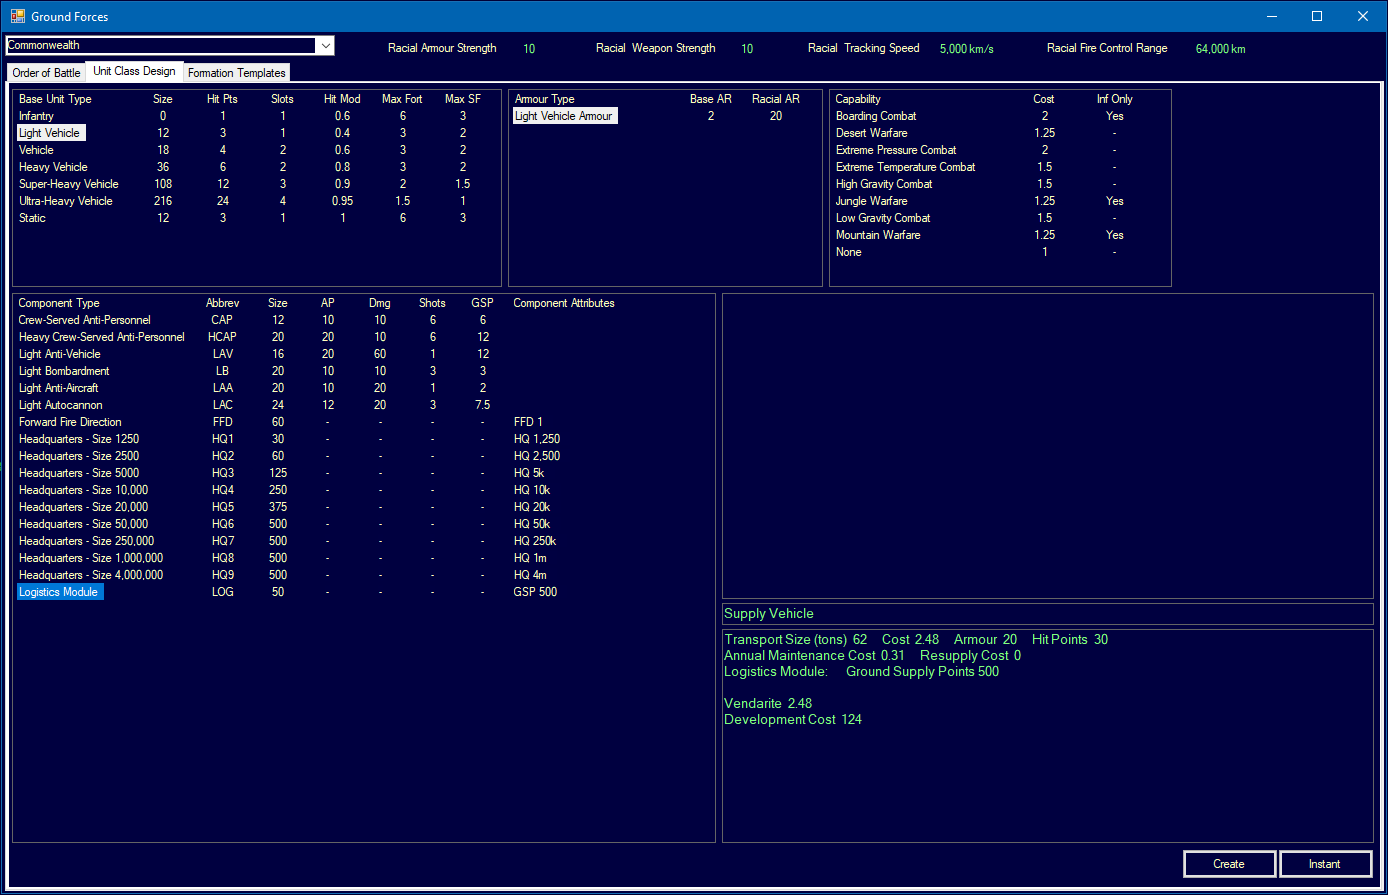
\includegraphics[width=0.95\linewidth]{images/SupplyVehicle}
		\caption[Supply Vehicle]{Supply Vehicle Example 1}
		\label{fig:supplyvehicle}
	\end{figure}
	
	Ground units with either logistics module can be added to any level of the ground force hierarchy, either embedded with the front line combat formations or held at a superior formation, such as a headquarters.
	
	Each Ground Unit has sufficient inherent supply points to fight ten rounds of combat (currently one round takes place every eight hours). After that point, only one quarter of units in a formation element that is out of supply will fire in each round. In addition, a formation with out of supply elements cannot use a field position of 'Front Line Attack' (more on this when I publish the full ground combat rules). However, if units with logistics modules are available, ground units can draw supply to both fight the current combat round and replenish supplies used in previous combat rounds.
	
	Ground Units will attempt to draw supply from the formation that sits highest in their hierarchy and is at the same population. If no supply is available, they will move down the hierarchy to their own parent formation, checking at each stage. However, when drawing supply from outside their own formation, units can only draw on logistic modules mounted on light vehicles. Logistics modules with an infantry base type can only supply their own formation.
	
	For example, a formation element of 10 tanks engaged in combat is part of an armoured formation with a brigade HQ formation above it and a division HQ formation above that. The tanks will check for a vehicle-based logistics element within the division formation first, then a vehicle-based logistics element within the brigade formation and finally either type of logistic element within their own parent formation. If no logistic elements are available, the tanks will use their inherent supply, although they can only use that inherent supply for ten combat rounds, unless resupplied. If a unit does not require a full resupply (for example, it still has sufficient inherent supply for eight combat rounds), it will only draw an appropriate fraction of its normal GSP requirement (in this case 20\%).
	
	When a formation element of logistics units provides supply, a number of units will be consumed based on the supply required. For example, assume the 10 tanks above each have a GSP requirement of 100, which is 1000 for the whole element. If they draw on a logistics element using light vehicles with normal logistics modules (which have 500 GSP each), two of those logistics vehicles would be consumed. When the GSP requirement does not neatly fit into the 500 point granularity, there is a chance of an additional logistics vehicle being consumed. This chance is dependent on the fraction of supplies required. For example, if there were 12 tanks with a requirement of 1200, then two logistic vehicles would be consumed and there is 40\% chance (200 / 500) than a third vehicle will be consumed. This adds an element of uncertainty, as supplies may be consumed faster or slower than normal (although it will average out over time), plus it avoids any tracking of partial supplies per vehicle.
	
	Below is an example of a Formation Template for a Brigade Headquarters that includes 50 Supply Vehicles.
	\begin{figure}[H]
		\centering
		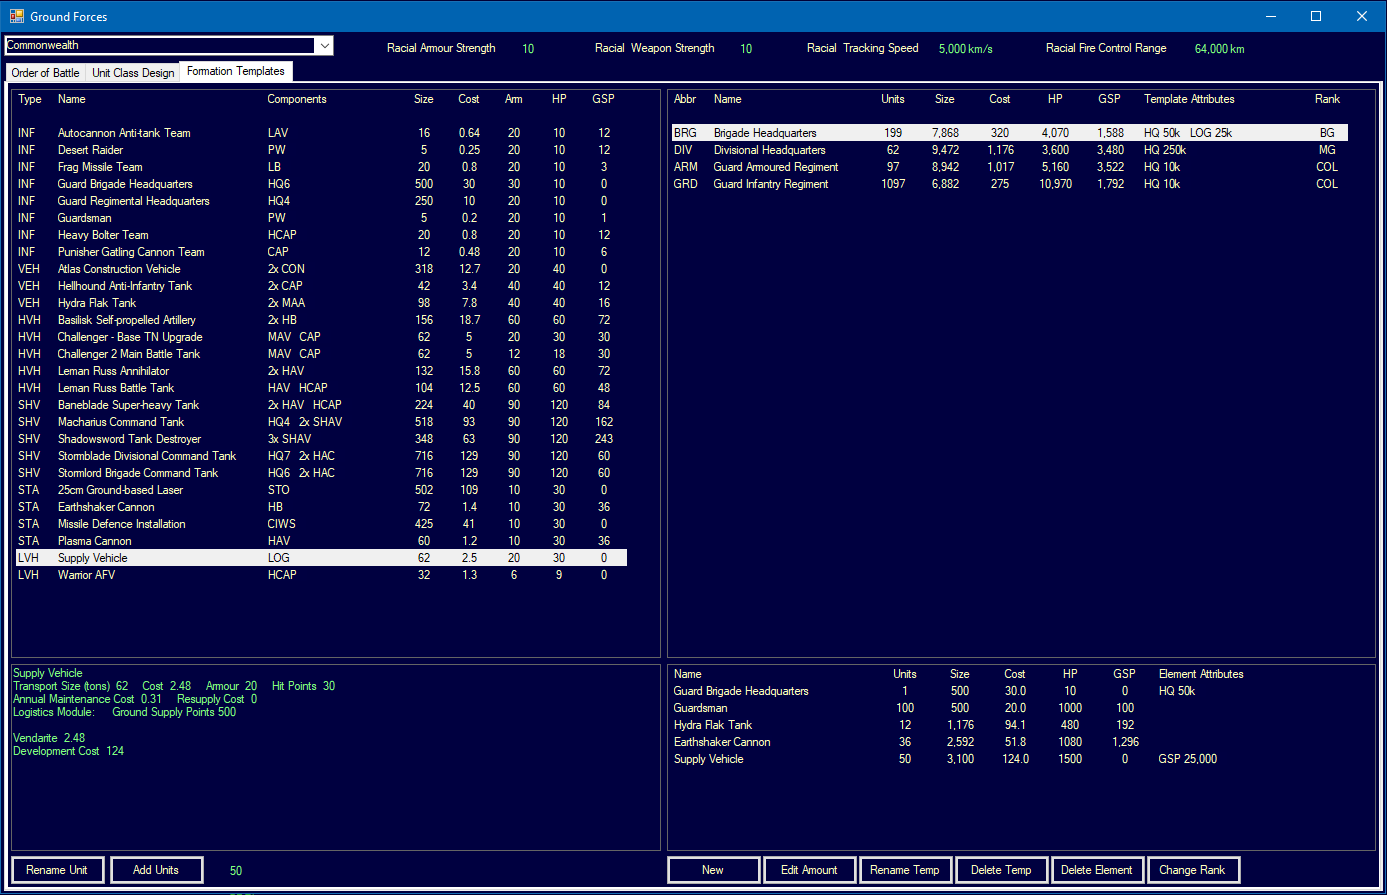
\includegraphics[width=0.95\linewidth]{images/SupplyVehicle2}
		\caption[Supply Vehicle]{Supply Vehicle Example 2}
		\label{fig:supplyvehicle2}
	\end{figure}

	Below is an order of battle for a divisional formation. At the divisional level are 240 Supply Vehicles, indicated by LOG 120k (120,000 supply points) in the Formation Attributes column, with smaller numbers within each brigade headquarters formation. The GSP column shows the resupply requirement for each formation or formation element. The total divisional organisation requires 40,338 GSP for a complete resupply and there are sufficient supply vehicles (410) in that organisation to resupply five times. With the inherent supply as well, the entire division can stay in combat for sixty rounds before additional supply vehicles are required.
	\begin{figure}[H]
		\centering
		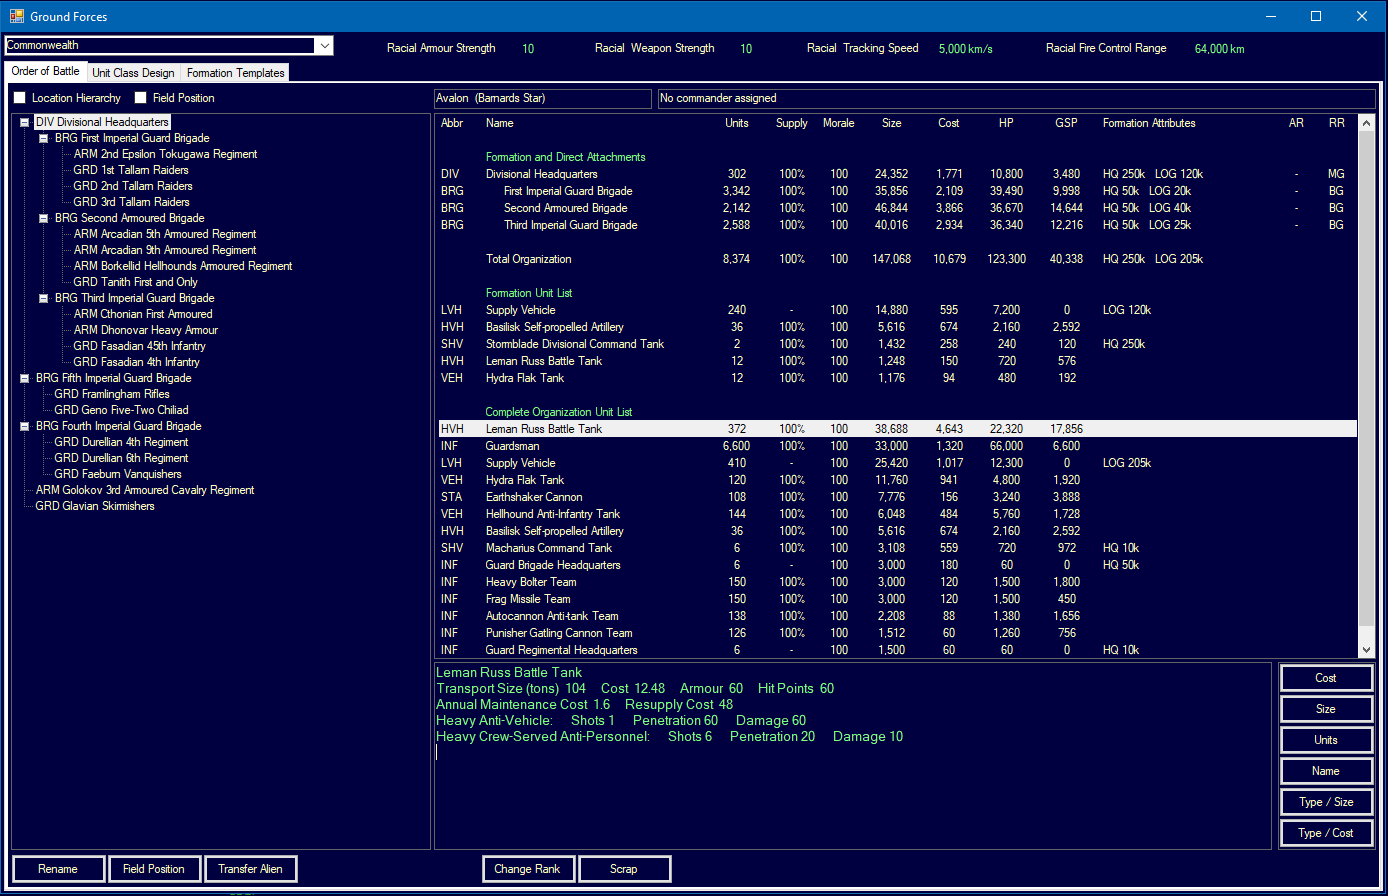
\includegraphics[width=0.95\linewidth]{images/SupplyVehicle3}
		\caption[Supply Vehicle]{Order of battle for divisional formation}
		\label{fig:supplyvehicle3}
	\end{figure}

	Finally here is a view of a single population, with the order of battle tab in Location mode.
	\begin{figure}[H]
		\centering
		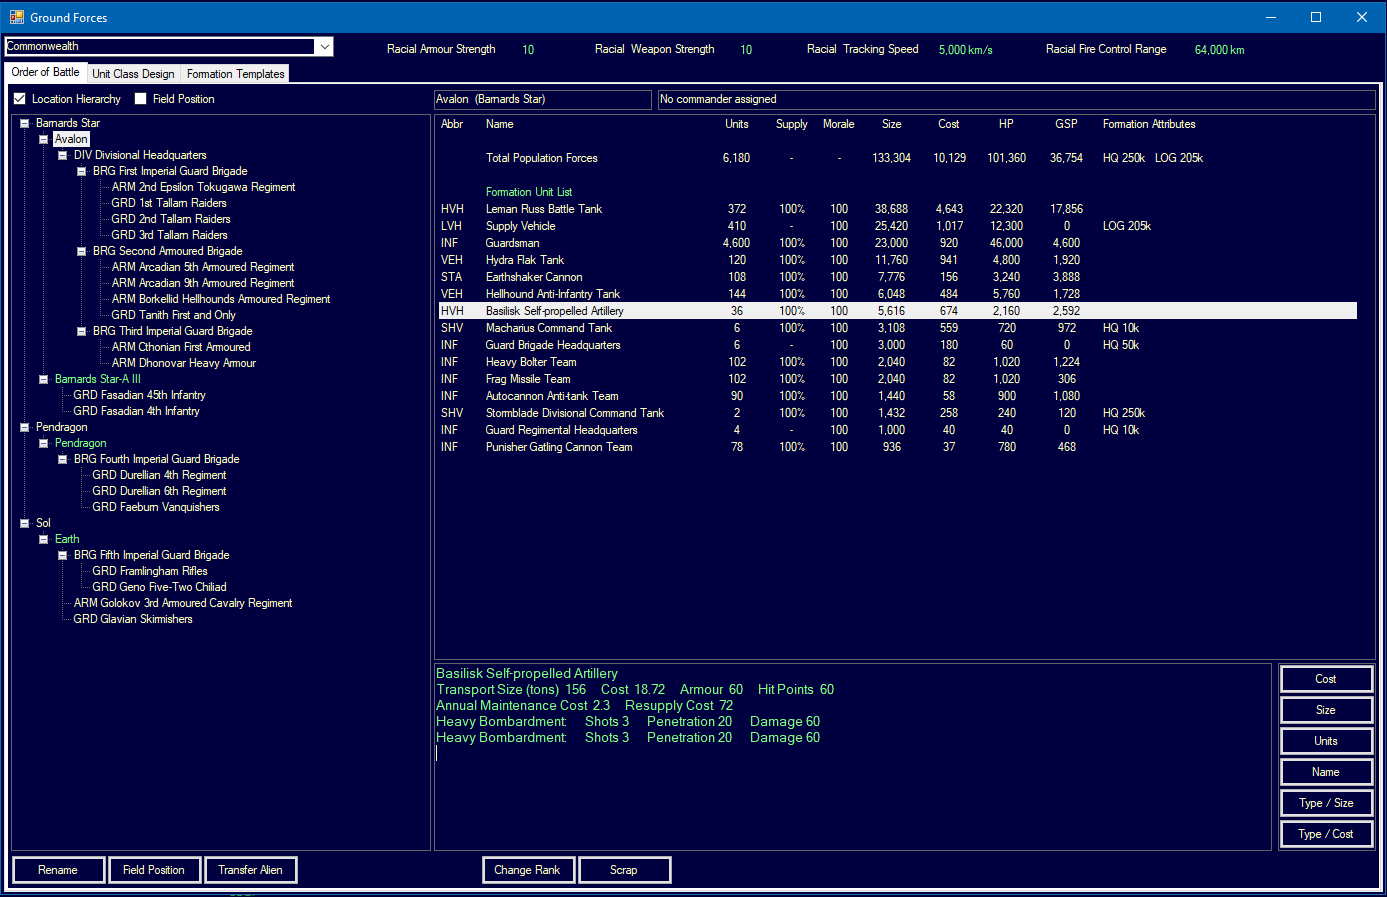
\includegraphics[width=0.95\linewidth]{images/SupplyVehicle4}
		\caption[Supply Vehicle]{Order of battle tab in Location mode}
		\label{fig:supplyvehicle4}
	\end{figure}
\end{document}